%%%%%%%%%%%%%%%%%%%%%%%%%%%%%%%%%% PROBLEM 1 %%%%%%%%%%%%%%%%%%%%%%%%%%%%%%%%%%
\section*{Problem 1}

A homogeneous U-235 reactor is operating at full power, 10,000 W/cm$^3$. 13\% of neutrons are absorbed in resonances, 2\% of all fission events are fast fissions, and 10\% of neutrons leak from the reactor. Assume 2.4 neutrons and 200 MeV are produced per fission, the fission cross section is 0.6 cm$^{-1}$, and the absorption cross section is 1 cm$^{-1}$.
\begin{enumerate}[a)]
\item Ignoring depletion, calculate the excess reactivity of this reactor.
\item The reactor scrams (immediately jumps to zero power). The plot below gives the negative reactivity as a function of time due to the accumulation of xenon in the reactor. Estimate at which point the reactor could no longer be returned to operation. About how long would this deadtime last?
\end{enumerate}
\begin{center}
\vspace{1cm}
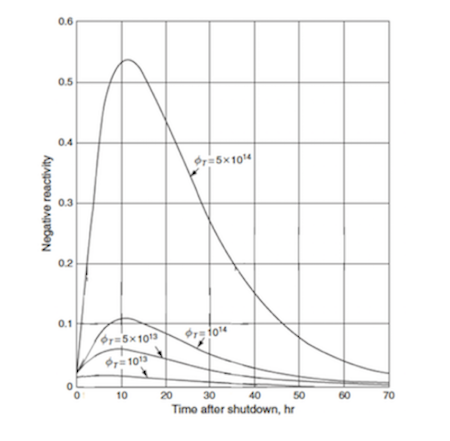
\includegraphics[width=12cm]{xenon-deadtime}
\end{center}
\vfill
$200\text{ MeV} = 3.204\times10^{-11}\text{ J}$

